\documentclass[a4paper,11pt,twocolumn]{article}
\usepackage{fancyhdr}
\usepackage{enumerate}
\usepackage{times}
\usepackage{mathptmx}
\usepackage{amsmath}
\usepackage{amsfonts}
\usepackage{amssymb}
\usepackage{tikz}
\usepackage[top=2cm, bottom=2cm, left=2cm, right=2cm]{geometry}

\setlength{\columnsep}{7mm}

\newcommand{\homeworkno}{3.3}
\pagestyle{fancy}
\lhead{Problem Solving: Homework \homeworkno}
\chead{}
\rhead{Chen Shaoyuan (161240004)}
\lfoot{}
\cfoot{\thepage}
\rfoot{}

\newcommand{\od}{\mathop{\mathrm{deg}}}

\allowdisplaybreaks[4]
\renewcommand{\labelenumi}{(\alph{enumi})}
\begin{document}
  \title{Problem Solving: Homework \homeworkno}
  \author{Name: Chen Shaoyuan \and Student ID: 161240004}
  \maketitle

  \section{[GC] Problem 5.3}
  \begin{enumerate}
    \item No. Here is a counterexample. \par
    \small
    \begin{center}
    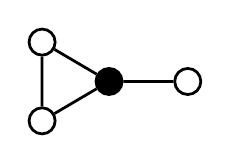
\begin{tikzpicture}[line width = 1pt,
                        solid/.style = {circle, draw, fill = black, minimum size = 0.1cm},
                        empty/.style = {circle, draw, fill = white, minimum size = 0.1cm}]
      \node [empty] (a1) at (0, 0){};
      \node [empty] (a2) at (0, 1){};
      \node [solid] (a3) at (0.85, 0.5){};
      \node [empty] (a4) at (1.85, 0.5){};
      \draw (a4) -- (a3) -- (a2) -- (a1) -- (a3);
    \end{tikzpicture}
    \end{center} \par
    \normalsize
    Consider the solid vertex. It lies on some cycle, however, it is a cut-vertex too.
    \item No. Here is a counterexample. \par
    \small
    \begin{center}
    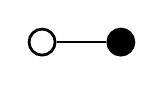
\begin{tikzpicture}[line width = 1pt,
                        solid/.style = {circle, draw, fill = black, minimum size = 0.1cm},
                        empty/.style = {circle, draw, fill = white, minimum size = 0.1cm}]
      \node [empty] (a1) at (0, 0){};
      \node [solid] (a2) at (1, 0){};
      \draw (a2) -- (a1);
    \end{tikzpicture}
    \end{center} \par
    \normalsize
    Cosider the solid vertex. It does not lie on any circle, but it is not a cut-vertex as well.
  \item No. Here is a counterexample. \par
  	\small
    \begin{center}
    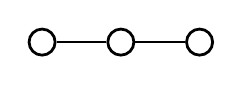
\begin{tikzpicture}[line width = 1pt,
                        solid/.style = {circle, draw, fill = black, minimum size = 0.1cm},
                        empty/.style = {circle, draw, fill = white, minimum size = 0.1cm}]
      \node [empty] (a1) at (0, 0){};
      \node [empty] (a2) at (1, 0){};
      \node [empty] (a3) at (2, 0){};
      \draw (a1) -- (a2) -- (a3);
    \end{tikzpicture}
    \end{center} \par
    \normalsize
    It has two end-vertices but only one cut-vertex.
  \item No. Consider the counterexample in (c), it has two bridges but only one cut-vertex.
  \end{enumerate}

  \section{[GC] Problem 5.4}
  Let $a$, $b$ be any two distinct vertices in $G - v$ that are connected in $\overline{G}$. We are going to prove that $a$ and $b$ are still connected in $\overline{G} - v$. \par
  Case 1: $a$ and $b$ are in different components of $G - v$. This means that $ab \notin E(G)$ and $ab \in E(\overline{G})$, and thus $ab \in E(\overline{G} - v)$. Therefore, $a$ and $b$ are still connected in $\overline{G} - v$. \par
  Case 2: $a$ and $b$ are in the same component of $G - v$. Since $G -v$ has at least two components, let $c$ be any vertex in the component of $G$ other than the one $a$ and $b$ are in. Therefore, $ac, cb \notin E(G)$, and $ac, cb \in E(\overline{G})$, and thus $ac, cb \in E(\overline{G})$. \par
  Therefore, removing $v$ in $\overline{G}$ does not make any two connected vertices $a, b (a, b \neq v)$ disconnected. This  means that $v$ is not a cut-vertex of $\overline{G}$.

  \section{[GC] Problem 5.6}
  The sufficiency is immediate by Corollary 5.2. We only have to prove the necessity. \par
  Let $v$ be any cut-vertex in $G$, and $a, b, c$ be neighbors of $v$. $a, b, c$ must in at least two different components of $G - v$, otherwise, $v$ is not a cut-vertex. Furthermore, there exists a component of $G - v$ that contains exactly one of $a, b, c$,  and without loss of generality, we assume the vertex is $a$. Suppose, to the contrary, that $va$ is not a bridge of $G$, then $va$ lies on some cycle by Theorem 4.1. Since $a, b, c$ are only neighbors of $v$, either $vb$ or $vc$ lies on $C$. Without loss of generality, assume $vb \in C$. Therefore, $C - {v}$ is an $a-b$ path, which contradicts Theorem 5.3. Therefore, $va$ is a bridge. \par

  \section{[GC] Problem 5.10}
  Note that a graph of size at least 2 contains at least 3 vertices, so Theorem 5.7 applies. \par
  Sufficiency: let $u, v$ be any two distinct vertices in $G$. Since $G$ is connectd, there exists a $u-v$ path, say $(u, w_1, w_2, \cdots, w_n, v)$. Since edges $uw_1, w_1w_2$, edges $w_1w_2, w_2w_3$, $\cdots$, edges $w_{n-1}w_n, w_nv$ lie on common cycles respectively, by Theorem 5.8 $uw_1, w_nv$ lie on  common cycle, and thus $u, v$ lie on same cycle. By Theorem 5.7 $G$ is nonseparable. \par
  Necessity: let $uv$, $vw$ be any two adjacent edges in nonseperable graph $G$. By Theorem 5.7, $u, w$ lie on common cycle $C$. If $v \in C$, then $uv, vw$ lie on common cycle $C$; otherwise, let $P$ be either $u-w$ path in cycle $C$, then $P \cup \{uv, vw\}$ forms a cycle where $uv, vw$ lie on.

  \section{[GC] Problem 5.11}
  By Theorem 5.3, we only have to show that, for every three distinct vertices $u, v, w \in G$, there exists a $u-w$ path that does not contain $v$. \par
  If $uw \in E(G)$, then the proof is done; otherwise, since $ \deg u = \deg w \geq n/2$ and $|V(G - \{u, w\})| = n - 2$, by pigeonhole principle, there exist two vertices $a, b$, such that $a, b$ are neighbors of both $u$ and $w$. At least one of $a$ and $b$ is not $v$, that vertex, along with $u$ and $v$, forms a $u-w$ path that does not contain $v$.

  \section{[GC] Problem 5.14}
  \begin{enumerate}
  	\item Since $G$ is connected, $G_1$ must be connected to some vertex in $G-G_1$. However, $G_1$ is not connected to $G-v-G_1$, because $G_1$ is a component of $G-v$. Therefore, only $v$ is connected to $G_1$, and $G[V(G_1) \cup \{v\}]$ is connected.
  	\item Consider the following graph $G$
  	\small
    \begin{center}
    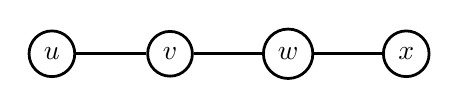
\begin{tikzpicture}[line width = 1pt,
                        solid/.style = {circle, draw, fill = black, minimum size = 0.1cm},
                        empty/.style = {circle, draw, fill = white, minimum size = 0.1cm}]
      \node [empty] (a1) at (0, 0){$u$};
      \node [empty] (a2) at (1.5, 0){$v$};
      \node [empty] (a3) at (3, 0){$w$};
      \node [empty] (a4) at (4.5, 0){$x$};
      \draw (a1) -- (a2) -- (a3) -- (a4);
    \end{tikzpicture}
    \end{center} \par
    \normalsize
    $v$ is a cut-vertex of $G$, and let $G_1$ be the component containing $w$ and $x$. $G[V(G_1) \cup \{v\}]$ is not a block, because $w$ is a cut-vertex.
  \end{enumerate}

  \section{[GC] Problem 5.15}
  Let $B$ be a block of $G$. \par
  (1) $\rightarrow$ (2): since $B$ is a nontrivial connected graph, it is induced by its edge set $E(B)$. Then we are going to prove $E(B)$ is an equivalent class resulting from the equivalence relation $R$ defined in Theorem 5.8. Since $B$ is connected, by Problem 5.10, for every two edges $e, f$, we have $e~R~f$. Let $e$ be any edge in $E(B)$, if $e~R~f$, then $f \in E(B)$. Otherwise, let $C$ be the common cycle where $e, f$ lie on. $G \cup C$ is a nonseparable graph by Problem 5.10,  and $G$ is a proper subgraph of $G \cup C$, which violates interpretation (1). Hence, $E(B)$ is an equivalent class of $R$. \par
  (2) $\rightarrow$ (1): since $E(B)$ is an equivalent class of $R$, by Problem 5.10, $B$ is nonseperable. $B$ can't be a proper subgraph of any other nonseparable graph $B'$ of $G$, otherwise, there exists $E(B)$ is a proper subset of $E(B')$ because $B'$ contains no isolated vertex, and for every $e, f \in E(B')$, $e~R~f$, which means $E(B)$ is not an equivalent class.

  \section{[GC] Problem 5.20}
  \begin{enumerate}
    \item Since $G$ is not $k$-connected $(k \leq n-2)$, $\kappa(G) \leq k-1$, and there exists a vertex cut $U_0$ with $|U_0| = \kappa(G)$. Let $C_1, C_2$ be any two components of $G - U_0$, and let $u, v$ be two vertices such that $u \in C_1$ and $v \in C_2$. Take any $k - 1 - \kappa(G)$ (possibly zero) vertices from $G - U_0 - \{u, v\}$ and add then to $U_0$, we obtain a vertex-cut $U$ with $|U| = k-1$.
    \item Since $G$ is not $k$-edge-connected, $\lambda(G) \leq k-1$, and there exists an edge cut $X_0$ with $|X_0| = \lambda(X_0)$. Since removing arbitrary number of edges does not decrease the number of components, we can take any $k-1-\lambda(G)$ (possibly zero) edges from $E(G) \backslash X$ and add them to $X_0$, and thus we obtain an edge cut $X$ with $|X| = k-1$.
  \end{enumerate}

  \section{[GC] Problem 5.22}
  \begin{enumerate}
    \item When $k = 1$, the proof is done. Otherwise, let $e = uv$. Consider every vertex subset $U$ of $G - e$ with $|U| = k-2$. Since $G$ is $k$-connected, if $u \in |U|$, $G - e - |U|$ is still connected; if $u \notin |U|$, $G - e - |U \cup \{u\}| = G - |U \cup \{u\}|$ is still connected. Therefore, $G-e$ is $(k-1)$-connected.
    \item When $k = 1$, the proof is done. Otherwise, consider every edge subset $X$ of $G-e$ with $|X| = k-2$, since $G-e-X =i G-(\{e\} \cup X)$ and $\{e\} \cup X$ is not an edge cut of $G$ because $G$ is $k$-edge-connected, $X$ is neither an edge cut of $G-e$. Therefore, $G-e$ is $(k-1)$-edge-connected.
  \end{enumerate}

  \section{[GC] Problem 5.30}
  $\overline{\kappa}(G) \geq \kappa(G)$, $\overline{\lambda}(G) \geq \lambda(G)$, $\overline{\kappa}(G) \leq \overline{\lambda}(G)$. \par
  The first two inequalities are what the definitions of $\overline{\kappa}$ and $\overline{\lambda}$ imply. Let's prove the third one. \par
  Let $H'$ be the subgraph of $G$ such that $\kappa(H') = \overline{\kappa}(G)$. By Theorem 5.11, $\overline{\kappa}(G) = \kappa(H') \leq \lambda(H')$. Since $\lambda(H') \leq \overline{\lambda}(G)$, we have $\overline{\kappa}(G) \leq \overline{\lambda}(G)$.

  \section{[GC] Problem 6.4}
  \begin{enumerate}
    \item $C_5$
    \small
    \begin{center}
    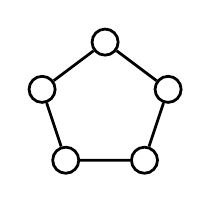
\begin{tikzpicture}[line width = 1pt,
                        solid/.style = {circle, draw, fill = black, minimum size = 0.1cm},
                        empty/.style = {circle, draw, fill = white, minimum size = 0.1cm}]
      \node [empty] (a1) at (0, 0){};
      \node [empty] (a2) at (1, 0){};
      \node [empty] (a3) at (1.3, 0.9){};
      \node [empty] (a4) at (0.5, 1.5){};
      \node [empty] (a5) at (-0.3, 0.9){};
      \draw (a1) -- (a2) -- (a3) -- (a4) -- (a5) -- (a1);
    \end{tikzpicture}
    \end{center} \par
    \normalsize
\item $C_6$
    \small
    \begin{center}
    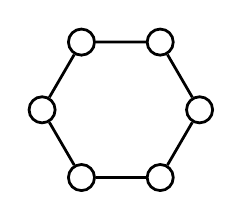
\begin{tikzpicture}[line width = 1pt,
                        solid/.style = {circle, draw, fill = black, minimum size = 0.1cm},
                        empty/.style = {circle, draw, fill = white, minimum size = 0.1cm}]
      \node [empty] (a1) at (0, 0){};
      \node [empty] (a2) at (1, 0){};
      \node [empty] (a3) at (-0.5, 0.86){};
      \node [empty] (a4) at (1.5, 0.86){};
      \node [empty] (a5) at (0, 1.72){};
      \node [empty] (a6) at (1, 1.72){};
      \draw (a1) -- (a2) -- (a4) -- (a6) -- (a5) -- (a3) -- (a1);
    \end{tikzpicture}
    \end{center} \par
    \normalsize
    \newpage
    \item $P_4$
    \small
    \begin{center}
    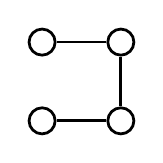
\begin{tikzpicture}[line width = 1pt,
                        solid/.style = {circle, draw, fill = black, minimum size = 0.1cm},
                        empty/.style = {circle, draw, fill = white, minimum size = 0.1cm}]
      \node [empty] (a1) at (0, 0){};
      \node [empty] (a2) at (1, 0){};
      \node [empty] (a3) at (1, 1){};
      \node [empty] (a4) at (0, 1){};
      \draw (a1) -- (a2) -- (a3) -- (a4);
    \end{tikzpicture}
    \end{center} \par
    \normalsize
    \item $P_2 \times P_3$
    \small
    \begin{center}
    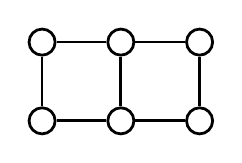
\begin{tikzpicture}[line width = 1pt,
                        solid/.style = {circle, draw, fill = black, minimum size = 0.1cm},
                        empty/.style = {circle, draw, fill = white, minimum size = 0.1cm}]
      \node [empty] (a1) at (0, 0){};
      \node [empty] (a2) at (1, 0){};
      \node [empty] (a3) at (1, 1){};
      \node [empty] (a4) at (0, 1){};
      \node [empty] (a5) at (2, 0){};
      \node [empty] (a6) at (2, 1){};
      \draw (a2) -- (a3) -- (a4) -- (a1) -- (a2) -- (a5) -- (a6) -- (a3);
    \end{tikzpicture}
    \end{center} \par
    \normalsize
    \item (the dashed edge is $e$)
    \small
    \begin{center}
    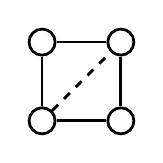
\begin{tikzpicture}[line width = 1pt,
                        solid/.style = {circle, draw, fill = black, minimum size = 0.1cm},
                        empty/.style = {circle, draw, fill = white, minimum size = 0.1cm}]
      \node [empty] (a1) at (0, 0){};
      \node [empty] (a2) at (1, 0){};
      \node [empty] (a3) at (1, 1){};
      \node [empty] (a4) at (0, 1){};
      \draw (a1) -- (a2) -- (a3) -- (a4) -- (a1);
      \draw [dashed] (a1) -- (a3);
    \end{tikzpicture}
    \end{center} \par
    \normalsize
  \end{enumerate}
  
  \section{[GC] Problem 6.5}
  It is $K_5$ with any of its edges removed.
  
  \section{[GC] Problem 6.6}
  Assume $G$ is $r$-regular. Since $G$ is not Eulerian, by Theorem 6.1, $r$ is odd, and thus $n$ is even. Therefore, $\overline{G}$ is $(n-1-r)$-regular graph, where $n-1-r$ is even. By Theorem 6.1, $\overline{G}$ is Eulerian.
  
  \section{[GC] Problem 6.13}
  \begin{enumerate}
    \item The following graph is not Hamiltonian, because it violates a necessary condition for a graph to be Hamiltonian (Theorem 6.5), if we take $S = \{v\}$.
    \small
    \begin{center}
    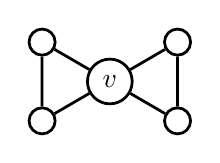
\begin{tikzpicture}[line width = 1pt,
                        solid/.style = {circle, draw, fill = black, minimum size = 0.1cm},
                        empty/.style = {circle, draw, fill = white, minimum size = 0.1cm}]
      \node [empty] (a1) at (0, 0){};
      \node [empty] (a2) at (0, 1){};
      \node [empty] (a3) at (0.86, 0.5){$v$};
      \node [empty] (a4) at (1.72, 0){};
      \node [empty] (a5) at (1.72, 1){};
      \draw (a3) -- (a1) -- (a2) -- (a3) -- (a4) -- (a5) -- (a3);
    \end{tikzpicture}
    \end{center} \par
    \normalsize
    \item The following graph is not Eulerian, because it has two odd vertices.
    \small
    \begin{center}
    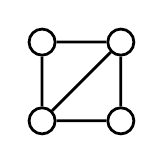
\begin{tikzpicture}[line width = 1pt,
                        solid/.style = {circle, draw, fill = black, minimum size = 0.1cm},
                        empty/.style = {circle, draw, fill = white, minimum size = 0.1cm}]
      \node [empty] (a1) at (0, 0){};
      \node [empty] (a2) at (0, 1){};
      \node [empty] (a3) at (1, 1){};
      \node [empty] (a4) at (1, 0){};
      \draw (a3) -- (a1) -- (a2) -- (a3) -- (a4) -- (a1);
    \end{tikzpicture}
    \end{center} \par
    \normalsize
    \item The same one as (b).
    \item $\quad$ \\
    \small
    \begin{center}
    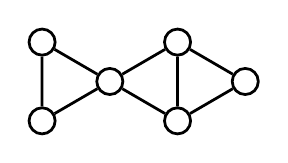
\begin{tikzpicture}[line width = 1pt,
                        solid/.style = {circle, draw, fill = black, minimum size = 0.1cm},
                        empty/.style = {circle, draw, fill = white, minimum size = 0.1cm}]
      \node [empty] (a1) at (0, 0){};
      \node [empty] (a2) at (0, 1){};
      \node [empty] (a3) at (0.86, 0.5){};
      \node [empty] (a4) at (1.72, 0){};
      \node [empty] (a5) at (1.72, 1){};
      \node [empty] (a6) at (2.58, 0.5){};
      \draw (a3) -- (a1) -- (a2) -- (a3) -- (a4) -- (a5) -- (a3);
      \draw (a4) -- (a6) -- (a5);
    \end{tikzpicture}
    \end{center} \par
    \normalsize
  \end{enumerate}
  
  \section{[GC] Problem 6.16}
  \begin{enumerate}
    \item We have proved in Problem 6.6 that if $G$ is not Eulerian, then $\overline{G}$ is Eulerian. If $G$ is Eulerian, then $r$ is even. Hence, $\overline{G}$ is $(n-1-r)$-regular, where $n-1-r$ is odd, which means $\overline{G}$ is not Eulerian. Therefore, either $G$ or $\overline{G}$ is Eulerian.
    \item If $G$ is not Hamiltonian, by Corollary 6.7, there exists a vertices $u$, such that
    $$ \deg u  = r < n / 2.$$
    Therefore, for each vertex $u'$ in $\overline{G}$,
    $$ \deg u'  = n - 1 - r > n/2 - 1 \geq n/2$$
    by Corollary 6.7, $\overline{G}$ is Hamiltonian. \par
    It is possible that both $G$ and $\overline{G}$ are Hamiltonian. (consider $C_6$)
  \end{enumerate}
  
  \section{[GC] Problem 6.21}
  Add a new vertex $u$ along with edges $uv (v \in G)$ to $G$, and let $G'$ denote the the resulting graph. It is obvious that for every pair of non- adjacent vertices $u, v \in G'$, $\deg_{G'} u + \deg_{G'} v \geq n + 1$. By Theorem 6.6, $G'$ contains a Hamiltonian cycle $C$. Removing $v$ and edges incident with $v$ from $C$ gives a Hamiltonian path of $G$.
\end{document}
